\documentclass[12pt,oneside]{amsbook}%,draft

\usepackage[italian]{babel}
\usepackage[utf8]{inputenc}
\usepackage{amsmath,amsthm}%
\usepackage{amsfonts}%
\usepackage{amssymb}%
\usepackage{mathrsfs}
\usepackage{graphicx,pdfsync}
\usepackage{ulem,color}

%----------------------------------------------------------
% Impaginazione ufficiale tesi
%\usepackage[a4paper,top=3cm,bottom=3.5cm,left=3.5cm,right=2.5cm]{geometry}
% impaginazione stampa bozze 
\usepackage[a4paper,top=2cm,bottom=2cm,textwidth=17cm]{geometry}

%,includehead,includefoot
\linespread{2}


%---------------------------------------------------------
% Gestione hyperlink
\usepackage[colorlinks=true,naturalnames=true,urlcolor=blue]{hyperref}

%% impostazioni per formattazione ambienti
\theoremstyle{plain}
\newtheorem{theorem}{Teorema}[chapter]
\newtheorem{lemma}{Lemma}[chapter]
\newtheorem{proposition}{Proposizione}[chapter]
\newtheorem{corollary}{Corollario}[chapter]
\newtheorem{fatto}{Fatto}

\newcounter{examples}

\theoremstyle{definition}
\newtheorem{definition}{Definizione}[chapter]
%\newtheorem{esempio}{Esempio}[examples]
\newtheorem{example}{Esempio}[chapter]

\theoremstyle{definition}
\newtheorem*{remark}{Osservazione}


%----------------------------------------------------------
\newcommand{\F}{\mathscr{F}}
\renewcommand{\P}{\mathbb{P}}


\begin{document}
\frontmatter
\begin {titlepage}
\begin{center}
UNIVERSIT\`A DEGLI STUDI DELL'INSUBRIA - COMO\\
Dipartimento di Scienza ed Alta Tecnologia\\
Corso di Laurea in Matematica
\end{center}
\vfill
\begin{figure}[h]
	\begin{center} 
		\scalebox{.2}{
\includegraphics{logo}} 
	\end{center} 
\end{figure}
\vfill
\begin{center}
\LARGE{Xxxxxxx Xxxxxxx Xxxxxx Xxxxxxxxxx}
\end{center}
\vfill
\vfill
\vfill
\begin{flushleft}
Relatore: dott. Andrea MARTINELLI\\
Correlatore: 
\end{flushleft}
\vfill
\begin{flushright}
Tesi di Laurea di\\
XXXXXXXXXXXXXXXXXXXXX\\
Matricola n. XXXXXX
\end{flushright}
\vfill
\begin{center}
Anno Accademico 20xx--20xx
\end{center}
\end{titlepage}

\tableofcontents



\chapter*{Introduzione}




\mainmatter

\chapter{A}

\begin{figure}[htbp]
\begin{center}
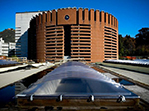
\includegraphics{figures/image}
\caption{default}
\label{default}
\end{center}
\end{figure}


\chapter{B}

\section{One}
Lorem ipsum dolor sit amet, consectetur adipiscing elit. Nunc ac nisi urna. Sed gravida felis vitae sapien eleifend, non varius libero auctor. Vestibulum nec lorem ac est lacinia lobortis quis non enim. Aenean consequat quam purus, in aliquet neque malesuada vel. Vivamus cursus laoreet libero eget vestibulum. Vestibulum in blandit dolor. Quisque ut mauris nibh. Cras consectetur egestas orci a tristique. Integer a lacinia dolor, vel convallis nisi. Donec eu ipsum pharetra, porta lorem sit amet, tincidunt justo. Fusce pulvinar efficitur urna eu consequat. Nullam at ligula sit amet dui dictum pharetra et eget nibh.

\section{Two}
Donec ullamcorper, elit sed iaculis efficitur, dolor erat porttitor metus, a maximus erat velit in nisi. Curabitur gravida eget lacus vel fermentum. Quisque ac vulputate diam. Vivamus porta fringilla lacinia. Aenean vestibulum aliquet erat ac congue. Morbi vulputate cursus lacus, et sollicitudin sem suscipit vitae. Quisque vestibulum libero vel mi venenatis consequat. Pellentesque aliquam, massa et porta suscipit, turpis libero bibendum leo, vel pulvinar est lectus eget urna. Vivamus ornare augue interdum nulla bibendum ornare. Mauris sit amet commodo est. Ut id mollis ligula.

\section{Three}
Nunc varius nunc id nulla faucibus, vel scelerisque nunc ultricies. Etiam tincidunt leo vel odio pulvinar iaculis. Pellentesque habitant morbi tristique senectus et netus et malesuada fames ac turpis egestas. Integer volutpat molestie quam et tristique. Donec a mauris convallis, eleifend ex id, ultricies ipsum. Sed viverra, urna dignissim pellentesque molestie, dolor eros rutrum diam, in convallis velit turpis ac nibh. Nam feugiat dui vel pretium cursus. Donec condimentum eros erat. In rutrum, velit ut convallis mollis, tortor ante facilisis metus, sed gravida nibh nisl ut ligula.

\section{Four}
Aliquam feugiat finibus sem et euismod. Nam porta dui ex, sit amet fermentum felis hendrerit vel. Duis scelerisque eget tortor ut iaculis. Nullam pharetra tortor quis feugiat auctor. Phasellus dui lectus, iaculis nec lacus ac, pellentesque auctor felis. Fusce ut tristique justo, vitae sollicitudin metus. Fusce nec tristique risus, sed fringilla augue. In hac habitasse platea dictumst. Pellentesque sed nunc et justo consectetur finibus non a nunc. Vestibulum ante ipsum primis in faucibus orci luctus et ultrices posuere cubilia curae; Donec ultricies facilisis quam ac luctus. Quisque non dolor eget dui rutrum sodales. Pellentesque habitant morbi tristique senectus et netus et malesuada fames ac turpis egestas. Pellentesque neque tortor, ultrices et rhoncus a, iaculis eget mi. Interdum et malesuada fames ac ante ipsum primis in faucibus. Pellentesque a ultrices sem.

Phasellus fermentum porta urna. Etiam auctor mauris sed vulputate hendrerit. Nunc facilisis tempus efficitur. Maecenas ornare eros quis leo auctor viverra. Suspendisse aliquam congue aliquet. Nam interdum at elit eget efficitur. Vestibulum gravida augue enim, sit amet hendrerit orci pellentesque id. Nam leo nunc, vehicula vitae eros ut, maximus ultricies justo.



\chapter{C}

\section{One}
Lorem ipsum dolor sit amet, consectetur adipiscing elit. Nunc ac nisi urna. Sed gravida felis vitae sapien eleifend, non varius libero auctor. Vestibulum nec lorem ac est lacinia lobortis quis non enim. Aenean consequat quam purus, in aliquet neque malesuada vel. Vivamus cursus laoreet libero eget vestibulum. Vestibulum in blandit dolor. Quisque ut mauris nibh. Cras consectetur egestas orci a tristique. Integer a lacinia dolor, vel convallis nisi. Donec eu ipsum pharetra, porta lorem sit amet, tincidunt justo. Fusce pulvinar efficitur urna eu consequat. Nullam at ligula sit amet dui dictum pharetra et eget nibh.

\section{Two}
Donec ullamcorper, elit sed iaculis efficitur, dolor erat porttitor metus, a maximus erat velit in nisi. Curabitur gravida eget lacus vel fermentum. Quisque ac vulputate diam. Vivamus porta fringilla lacinia. Aenean vestibulum aliquet erat ac congue. Morbi vulputate cursus lacus, et sollicitudin sem suscipit vitae. Quisque vestibulum libero vel mi venenatis consequat. Pellentesque aliquam, massa et porta suscipit, turpis libero bibendum leo, vel pulvinar est lectus eget urna. Vivamus ornare augue interdum nulla bibendum ornare. Mauris sit amet commodo est. Ut id mollis ligula.

\section{Three}
Nunc varius nunc id nulla faucibus, vel scelerisque nunc ultricies. Etiam tincidunt leo vel odio pulvinar iaculis. Pellentesque habitant morbi tristique senectus et netus et malesuada fames ac turpis egestas. Integer volutpat molestie quam et tristique. Donec a mauris convallis, eleifend ex id, ultricies ipsum. Sed viverra, urna dignissim pellentesque molestie, dolor eros rutrum diam, in convallis velit turpis ac nibh. Nam feugiat dui vel pretium cursus. Donec condimentum eros erat. In rutrum, velit ut convallis mollis, tortor ante facilisis metus, sed gravida nibh nisl ut ligula.

\section{Four}
Aliquam feugiat finibus sem et euismod. Nam porta dui ex, sit amet fermentum felis hendrerit vel. Duis scelerisque eget tortor ut iaculis. Nullam pharetra tortor quis feugiat auctor. Phasellus dui lectus, iaculis nec lacus ac, pellentesque auctor felis. Fusce ut tristique justo, vitae sollicitudin metus. Fusce nec tristique risus, sed fringilla augue. In hac habitasse platea dictumst. Pellentesque sed nunc et justo consectetur finibus non a nunc. Vestibulum ante ipsum primis in faucibus orci luctus et ultrices posuere cubilia curae; Donec ultricies facilisis quam ac luctus. Quisque non dolor eget dui rutrum sodales. Pellentesque habitant morbi tristique senectus et netus et malesuada fames ac turpis egestas. Pellentesque neque tortor, ultrices et rhoncus a, iaculis eget mi. Interdum et malesuada fames ac ante ipsum primis in faucibus. Pellentesque a ultrices sem.

Phasellus fermentum porta urna. Etiam auctor mauris sed vulputate hendrerit. Nunc facilisis tempus efficitur. Maecenas ornare eros quis leo auctor viverra. Suspendisse aliquam congue aliquet. Nam interdum at elit eget efficitur. Vestibulum gravida augue enim, sit amet hendrerit orci pellentesque id. Nam leo nunc, vehicula vitae eros ut, maximus ultricies justo.





%\begin{thebibliography}{9}
%\end{thebibliography}





\end {document}
